
\section{Elements and Transformations}
\label{sec:elements}
\subsection{Defining the Reference Elements}

In this section the three basic reference elements, for one, two and three dimensions, are defined.
They could be described as n-cuboid shapes because they are shaped like the cells of rectilinear structured grids.
For consistency with the implementation, the indices start at zero (\texttt{C++} indexing).

\subsubsection{Edge Element (1D)}

In a one-dimensional mesh, an element is a line segment or an edge.
The reference edge element is one-dimensional and starts at 0 and ends at 1.
The first vertex with index 0 is at $0$, and the second vertex with index 1 is at $1$.
the indexing is visualized in figure \ref{fig:edge_element}.

\begin{figure}[h]
    \vspace{0.5cm}
    \centering
    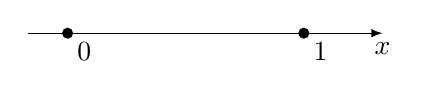
\begin{tikzpicture}
        \draw[-latex] (-0.5,0,0) -- (4,0,0) node[below] {$x$};

        % Define the vertices of the cube
        \coordinate (A) at (0, 0);
        \coordinate (B) at (3, 0);

        % Draw the edges of the cube
        \draw[black] (A) -- (B) -- cycle;

        % Draw the vertices of the cube
        \fill[black] (A) circle (2pt);
        \fill[black] (B) circle (2pt);

        % Label the vertices
        \node[below right] at (A) {0};
        \node[below right] at (B) {1};
    \end{tikzpicture}
    \caption{Illustration of the local vertex numbering on the reference edge element (1D).}
    \label{fig:edge_element}
\end{figure}

\subsubsection{Quadrilateral Element (2D)}

The 2D structured grid cells can be described by a quadrilateral. For rectilinear grids
those cells are rectangular.
However, the quadrilateral reference element in this framework aims to describe quadrilaterals,
which include parallelograms and by definition every closed, non-degenerate shape with four vertices.

The local vertices are ordered according to the right-hand rule.
The first vertex of the reference element is at $(0,0)$ and has index 0.
The second vertex of the reference element is located at $(1,0)$ and has index 1.
The vertex with index 2 is at $(1, 1)$ and the last vertex with index 3 is at $(0,1)$.
See figure \ref{fig:quad_element} for an illustration of the vertex indexing.

\begin{figure}[h]
    \centering
    \begin{tikzpicture}
        \draw[-latex] (-0.5,0,0) -- (4,0,0) node[below] {$x$};
        \draw[-latex] (0,-0.5,0) -- (0,4,0) node[above right] {$y$};

        % Define the vertices of the cube
        \coordinate (A) at (0, 0);
        \coordinate (B) at (3, 0);
        \coordinate (C) at (3, 3);
        \coordinate (D) at (0, 3);

        % Draw the edges of the cube
        \draw[black] (A) -- (B) -- (C) -- (D) -- cycle;

        % Draw the vertices of the cube
        \fill[black] (A) circle (2pt);
        \fill[black] (B) circle (2pt);
        \fill[black] (C) circle (2pt);
        \fill[black] (D) circle (2pt);

        % Label the vertices
        \node[below right] at (A) {0};
        \node[below right] at (B) {1};
        \node[below right] at (C) {2};
        \node[below right] at (D) {3};
    \end{tikzpicture}
    \caption{Illustration of the local vertex numbering on a quadrilateral element (2D).}
    \label{fig:quad_element}
\end{figure}

\subsubsection{Hexahedral Element (3D)}

Three-dimensional structured grids have hexahedral grid cells.
In rectilinear structured grids from IPPL, the cells can be described as bricks or rectangular cuboids.
The indexing follows the indexing from FEMSTER \cite{castillo_femster_2005}.
See figure \ref{fig:hex_element} for an illustration.

\begin{figure}[h]
    \centering
    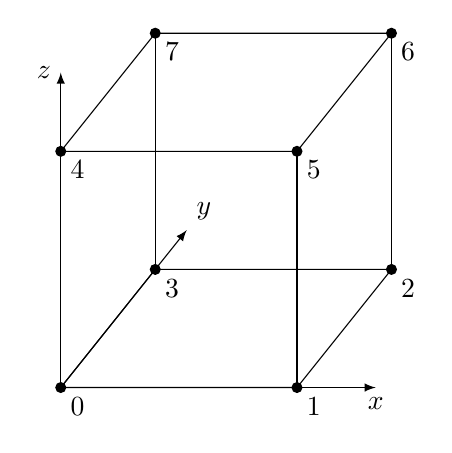
\begin{tikzpicture}[x={(1cm,0cm)}, y={(0.4cm,0.5cm)}, z={(0cm,1cm)}]
        \draw[-latex] (0,0,0) -- (4,0,0) node[below] {$x$};
        \draw[-latex] (0,0,0) -- (0,4,0) node[above right] {$y$};
        \draw[-latex] (0,0,0) -- (0,0,4) node[left] {$z$};

        % Define the vertices of the cube
        \coordinate (A) at (0, 0, 0);
        \coordinate (B) at (3, 0, 0);
        \coordinate (C) at (3, 3, 0);
        \coordinate (D) at (0, 3, 0);
        \coordinate (E) at (0, 0, 3);
        \coordinate (F) at (3, 0, 3);
        \coordinate (G) at (3, 3, 3);
        \coordinate (H) at (0, 3, 3);

        % Draw the edges of the cube
        \draw[black] (A) -- (B) -- (C) -- (D) -- cycle;
        \draw[black] (E) -- (F) -- (G) -- (H) -- cycle;
        \draw[black] (A) -- (E);
        \draw[black] (B) -- (F);
        \draw[black] (C) -- (G);
        \draw[black] (D) -- (H);

        % Draw the vertices of the cube
        \fill[black] (A) circle (2pt);
        \fill[black] (B) circle (2pt);
        \fill[black] (C) circle (2pt);
        \fill[black] (D) circle (2pt);
        \fill[black] (E) circle (2pt);
        \fill[black] (F) circle (2pt);
        \fill[black] (G) circle (2pt);
        \fill[black] (H) circle (2pt);

        % Label the vertices
        \node[below right] at (A) {0};
        \node[below right] at (B) {1};
        \node[below right] at (C) {2};
        \node[below right] at (D) {3};
        \node[below right] at (E) {4};
        \node[below right] at (F) {5};
        \node[below right] at (G) {6};
        \node[below right] at (H) {7};
    \end{tikzpicture}
    \caption{Illustration of the local vertex numbering on a hexahedral element (3D).}
    \label{fig:hex_element}
\end{figure}

\subsection{Transformations}
\label{sec:transformations}

In order to compute the values of the shape functions on the reference element $\hat{K}$
and transform them back to the global element $K$, we need a function that maps the global element to the reference element.
For this, we define the transformation function $\mat{\Phi}_K$ below.

\begin{definition}[Transformation Function]
    The transformation function  $\mat{\Phi}_K$ maps points from the local coordinate system of the reference element $\hat{K}$ to
    the global coordinate system of the global element $K$:
    \begin{align}
        \mat{\Phi}_K: \hat{K} \mapsto K.
    \end{align}
    To transform a point $\hat{\vec{x}} \in \hat{K}$ to its point in the global coordinate system $\vec{x} \in K$ we use:
    \begin{align}
        \vec{x} & = \mat{\Phi}_K(\hat{\vec{x}}).
    \end{align}
    This is called a local-to-global transformation.

    The opposite from $\vec{x} \in K$ to $\hat{\vec{x}} \in \hat{K}$ is the global-to-local transformation using the inverse
    of the transformation function $\mat{\Phi}^{-1}_K$:
    \begin{align}
        \hat{\vec{x}} & = \mat{\Phi}^{-1}_K(\vec{x}).
    \end{align}
\end{definition}

At the time of writing, IPPL only supports rectilinear structured grid meshes for which affine transformations are sufficient.
Thus, only affine transformations were implemented, instead of more general bilinear transformations.
For more information on how to update this implementation to use bilinear transformations instead, see
section \ref{sec:bilinear_transformations} in the Appendix.

The difference between the bilinear and affine transformations is that the affine transformations can only
handle transformations to parallelograms whereas bilinear transformations cover all possible transformations for quadrilaterals.

\begin{definition}[Affine Transformation]
    \label{def:affine_trans}
    An affine transformation combines a linear transformation and a translation and is defined as
    \begin{align}
        \mat{\Phi}_K(\hat{\vec{x}}) = \mat{F}_K \hat{\vec{x}} + \vec{\tau}_K,
    \end{align}
    where $\hat{\vec{x}}$ is the point to transform in the reference coordinate system, $\mat{F}_K$ is
    the transformation matrix and $\vec{\tau}_K$ is the translation vector.
\end{definition}

Also, on a side note, not implementing bilinear transformations means that technically the \texttt{QuadrilateralElement} class currently only supports
parallelograms instead of all quadrilaterals.
Similarly, the \texttt{HexahedralElement} does not support transformations to all hexahedrons.

Also, since we assume rectilinear grids, we can go one step further because the linear transformation in the affine transformation
can be simplified even more to just a scaling transformation.
Thus we can use a transformation matrix as follows:
\begin{align}
    \label{eq:scaling_transform_mat}
    \mat{F}_K := \begin{bmatrix}
                     \boldsymbol{v}^1_x - \boldsymbol{v}^0_x & 0                                       & 0                                       \\
                     0                                       & \boldsymbol{v}^2_y - \boldsymbol{v}^0_y & 0                                       \\
                     0                                       & 0                                       & \boldsymbol{v}^4_z - \boldsymbol{v}^0_z
                 \end{bmatrix}.
\end{align}
Equation \ref{eq:scaling_transform_mat} is the scaling transformation matrix for three dimensions,
where $\vec{v}^i \in \R^d$ is the $i$-th local vertex of the element with $d$ entries for each dimension.

\begin{figure}[h]
    \centering
    \begin{tikzpicture}

        \draw[->] (0,0) -- (2.4,0) node[at end, right] {$\hat{x}$};
        \draw[->] (0,0) -- (0,2.4) node[at end, above] {$\hat{y}$};
        \draw[step=2cm,black,thin] (0,0) grid (2,2);
        \node[black, font=\small] at (1,1) {$\hat{K}$};

        \draw[->] (3,1.5) -- (5,1.5) node[midway, above] {$\mat{\Phi}_K$};
        \draw[->] (5,1) -- (3,1) node[midway, below] {$\mat{\Phi}^{-1}_K$};

        \draw[step=2cm,gray,very thin] (6,0) grid (12.4,5.4);
        \draw[->] (6,0) -- (12.4,0) node[at end, right] {$x$};
        \draw[->] (6,0) -- (6,5.4) node[at end, above] {$y$};

        \draw[thin,black] (7.8,1.2) -- (11,1.2);
        \draw[thin,black] (11,1.2) -- (11,3.6);
        \draw[thin,black] (7.8,1.2) -- (7.8,3.6);
        \draw[thin,black] (7.8,3.6) -- (11,3.6);
        \node[black, font=\small] at (9.9,2.4) {$K$};

        \fill[black] (7.8,1.2) circle (1.5pt);
        \node[black, font=\small, anchor=north west] at (7.8,1.2) {$\vec{v}^0$};
        \fill[black] (11,1.2) circle (1.5pt);
        \node[black, font=\small, anchor=north west] at (11,1.2) {$\vec{v}^1$};
        \fill[black] (7.8,3.6) circle (1.5pt);
        \node[black, font=\small, anchor=north west] at (7.8,3.6) {$\vec{v}^2$};
        \fill[black] (11,3.6) circle (1.5pt);
        \node[black, font=\small, anchor=north west] at (11,3.6) {$\vec{v}^3$};

        \draw[->] (6,0) -- (7.8,1.2) node[midway, above] {$\vec{\tau}_K\,$};
    \end{tikzpicture}
    \caption{Illustration of a 2D transformation (scaling and translation only).}
    \label{fig:affine_trans}
\end{figure}


\subsubsection{Applying Affine Tranformations}

In this subsection, the transformation will be applied to integrals and gradients.

First, we define how to apply the transformation to functions using the \emph{pullback} operation.

\begin{definition}[Pullback]
    The pullback $\mat{\Phi}_K^* f$ of a function $f$ is defined as \cite{hiptmair_numerical_2023}:

    \begin{align}
        \label{}
        (\mat{\Phi}_K^* f)(\hat{\vec{x}}) := f(\mat{\Phi}_K(\hat{\vec{x}})), \quad \hat{\vec{x}} \in \hat{K}.
    \end{align}

    It applies the transformation function $\mat{\Phi}_K$ to the input of the function $f$.
\end{definition}

\begin{definition}[Transformation Jacobian]
    The \emph{Transformation Jacobian} is defined as \cite{hiptmair_numerical_2023}:
    \begin{align}
        \mathbf{D\Phi}_K(\hat{\boldsymbol{x}})
        = \left[ \frac{\partial (\mathbf{\Phi}_K(\hat{\boldsymbol{x}}))_i}{\partial \boldsymbol{x}_j} \right]^d_{i,j = 1}.
    \end{align}
\end{definition}

In this work, with the simplifications applied from before, the Jacobian $\mat{D \Phi}_K$ is equal to the transformation matrix:
\begin{align}
    \mathbf{D\Phi}_K(\hat{\boldsymbol{x}}) = \mat{F}_K.
\end{align}

The pullback can be applied to the gradient of a function as follows:

\begin{align}
    \mat{\Phi}_{K}^{*}(\nabla_{\vec{x}} u)(\hat{\vec{x}})
     & = (\mat{D \Phi}_{K}(\hat{\vec{x}}))^{-\top}(\nabla_{\hat{\vec{x}}}(\mat{\Phi}^{*}_K u))(\hat{\vec{x}}) \\
     & = (\mat{D \Phi}_{K}(\hat{\vec{x}}))^{-\top}(\nabla_{\hat{\vec{x}}}u)(\mat{\Phi}_K(\hat{\vec{x}})),
\end{align}
with the notation: $\mat{S}^{-\top} := (\mat{S}^{-1})^\top = (\mat{S}^\top)^{-1}$.

Also, the inverse of the Transformation Jacobian is equal to the inverse of the transformation matrix:
\begin{align}
    \mathbf{D\Phi}_K^{-1}(\hat{\boldsymbol{x}}) = \mat{F}_K^{-1}.
\end{align}

The determinant of the Transformation Jacobian is therefore also equal to the determinant of the transformation matrix:

\begin{align}
    |\det \mathbf{D\Phi}_K(\hat{\boldsymbol{x}})| = |\det \mat{F}_K|.
\end{align}

\subsection{Element classes}

The \texttt{Element} class is the base class for all the reference elements.
The reference element classes that inherit from it, define the indexing and position of the local vertices.
They also define the transformation functions for the local-to-global transformations.

The base \texttt{Element} class is abstract and dimension-independent and it takes in arguments for the
dimension \texttt{Dim}, as well as the datatype \texttt{T} and the number of
vertices \texttt{NumVertices}. The number of vertices is required at compile time
to define the size of the IPPL Vector, which also takes the size as a template
argument at compile time.

For now, transformations to lower dimensions are not supported.
Therefore the dimension template argument has to have the same dimension as the mesh.
